\chapter{Introduction to Information Retrieval}
In this course we will strongly consider \emph{search engines}, but \emph{information retrieval} is not
only consider on search engines, so a definition of information retrieval is the following

\begin{defi}
Information retrieval is finding material (usually documents) of unstructured nature that satisfies
an information need from within large collections
\end{defi}
An information need is the topic about which the user desires to know more, and is differentiated from a query,
which is what the user conveys to the computer in an attempt to communicate the information need.

As defined in this way, information retrieval used to be an activity that only a few people engaged in:
reference librarians, paralegals, and similar professional searchers, but now the world has changed,
and hundreds of millions of people engage in information retrieval every day when 
they use a web search engine or search their email.

Information retrieval systems can also be distinguished by the scale at
which they operate, and it is useful to distinguish three prominent scales.
In web search, the system has to provide search over billions of documents
stored on millions of computers. Distinctive issues are needing to gather
documents for indexing, being able to build systems that work efficiently
at this enormous scale, and handling particular aspects of the web, such as
the exploitation of hypertext

In between is the space of enterprise,
institutional, and domain-specific search, where retrieval might be provided for
collections such as a corporation’s internal documents, a database of patents,
or research articles on biochemistry. In this case, the documents will typically be stored on
centralized file systems and one or a handful of dedicated
machines will provide search over the collection

Data available and considered can be from different nature, so we have the following classification:
\begin{description}
    \item [Structured data: ] are data that tends to refer to tables and typically allows numerical range
                              and exact match (for text) queries, like for example "Salary < 60000 AND Manager = Smith".
    \item [Semistructured data (XML/JSON): ] type of data where are available some structured aspects, like know
                                             the name of a document, chapter or paragraph, so it facilitate some
                                             semi-structured search like 
                                             "Title contains data AND Bullets contain search".

    \item [Unstructured data: ] Typically refers to free text, and allows keyword queries including operators and
                                more sophisticated “concept” queries like find all web pages dealing with drug abuse.

                                Is the classic model for searching text documents, so we more concentrate on this
                                type of data.
\end{description}
We consider now the search engines, that are defined as 
\begin{defi}
A search engine is a software system that is designed to carry out search, which means to search page 
in a systematic way for particular information specified in a textual search query.\newline
The search results are generally presented in a line of results, often referred to as search engine results pages 
and the information may be a mix of links to pages, images, videos, infographics, articles, research papers,
and other types of files.
\end{defi}
Search engines are not only web search engine but contains also social network (Facebook), streaming site (Netflix),
Maps (OpenStreetMap) and work finder (Linkedin) and we have 5 generations of search engines:
\begin{description}
    \item [Zero generation: ] introduced on 1991, where was used only metadata added by users
    \item [First generation: ] introduced on 1995-1997 and used only on-page web-text data, as can be seen on 
                               figure \ref{img:altavista}.
                               \begin{figure}
                                \end{figure}
    \item [Second generation: ] introduced on 1998 by Google, use off-page, web-graph data, where it
                                use \emph{anchor texts} (how people refer to the page) and \emph{links}, that
                                strongly improve the usability and utility of a search engine.
                                An example of second generation search engine can be viewed on figure \ref{img:google}.
                                \begin{figure}
				    \begin{subfigure}{0.6\textwidth}
                                    	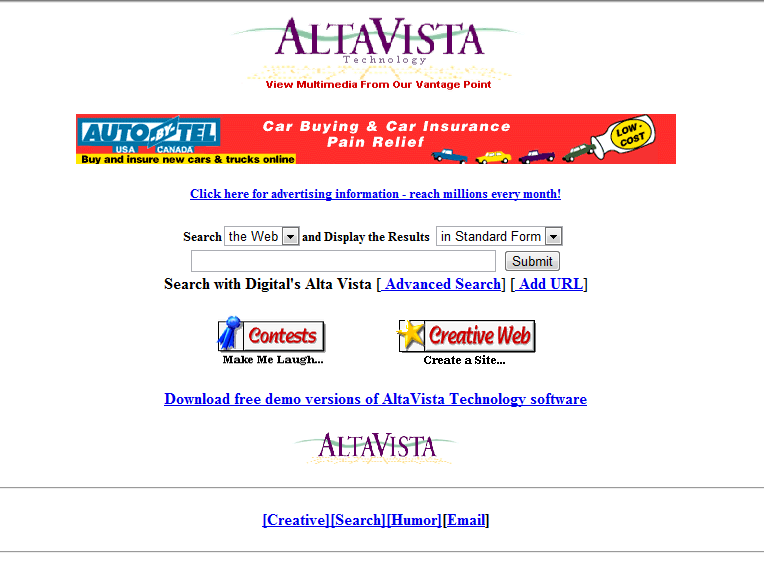
\includegraphics[width=0.6\textwidth]{Images/altavista}
                                    	\caption{Altavista search engine web page}
                                    	\label{img:altavista}
				    \end{subfigure}
				    \begin{subfigure}{0.6\textwidth}
                                    	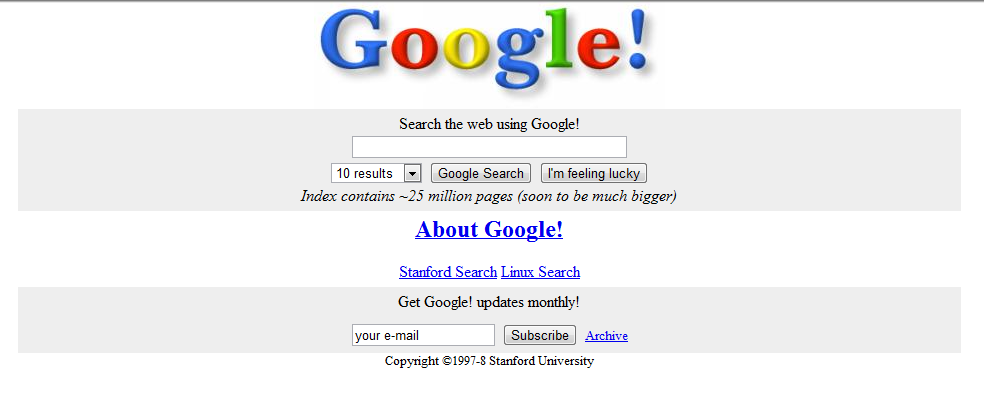
\includegraphics[width=0.8\textwidth]{Images/google}
                                    	\caption{Google search engine on 1998}
                                    	\label{img:google}
				    \end{subfigure}
				    \caption{Some example of Search Engine}
				    \label{img:generationSearch}
                                \end{figure}
    \item [Third generation: ] introduced on $2005$, it start to answer "the need behind the query" and are
                               added more sources, like maps, images, news, wikipedia and so on. 

    \item [Fourth generation: ] introduced on $2012$, it strongly concern about \emph{knowledge graph} defined as
                                \begin{defi}
                                Knowledge graph is a knowledge base used by Google and its services to enhance
                                its search engine's results with information gathered from a variety of sources.\newline
                                The information is presented to users in an infobox next to the search results.
                                \end{defi}
                                An example of knowledge graph can be viewed on figure \ref{img:knowledgeGraph} and
                                knowledge graph also permit to transform word to concept, that can provide more
                                information and provide more accurate results on user query, as we can see on 
                                figure \ref{img:leonardo} as we can viewed the phrase "Leonardo is the scientist
                                that has painted the Mona Lisa". \newline
                                With Knowledge graph is also possible to consider \emph{polysemy} and 
                                \emph{sinonimy} word, so at example is possible recognise that "Microsoft's browser"
                                and "Internet explorer" represent the same concept.
                                \begin{figure}
                                    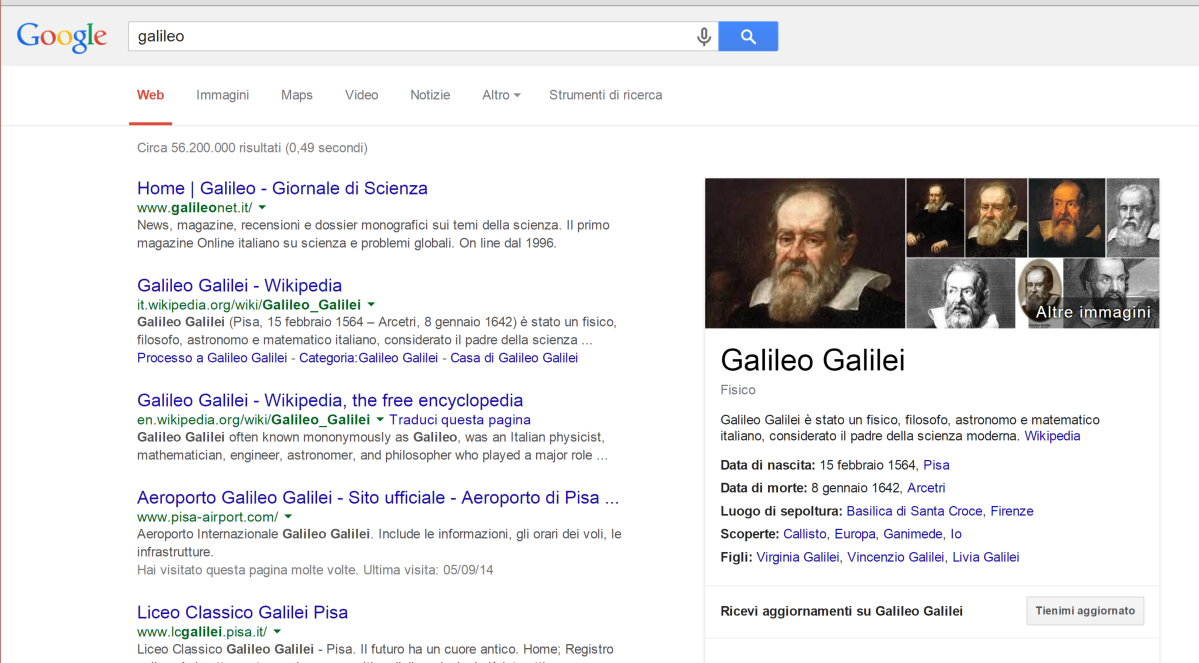
\includegraphics[width=0.6\textwidth]{Images/knowledgeGraph}
                                    \caption{A Google search with knowledge graph}
                                    \label{img:knowledgeGraph}
                                \end{figure}
                                \begin{figure}
                                    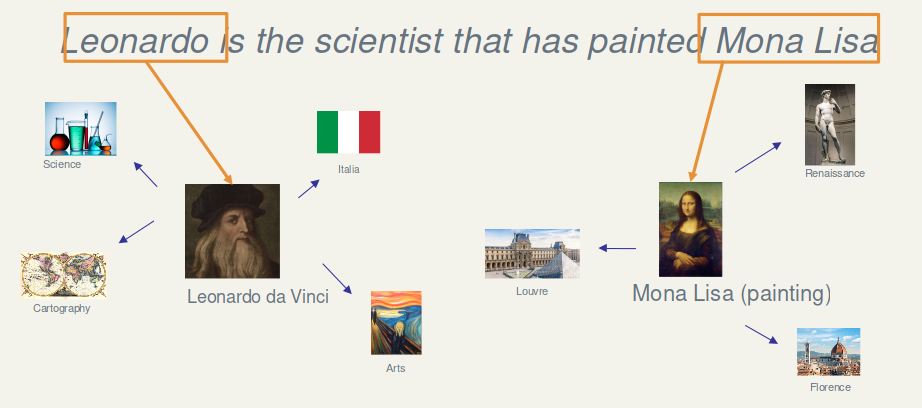
\includegraphics[width=0.6\textwidth]{Images/leonardo}
                                    \caption{an example of transition from word to concept with the phrase
                                             "Leonardo is the scientist that has painted the Mona Lisa"}
                                    \label{img:leonardo}
                                \end{figure}
\end{description}
In figure \ref{img:googleEvolution} is possible to notice which was the evolution on Google search engine.

\begin{figure}
    \caption{Google search evolution}
    \label{img:googleEvolution}
    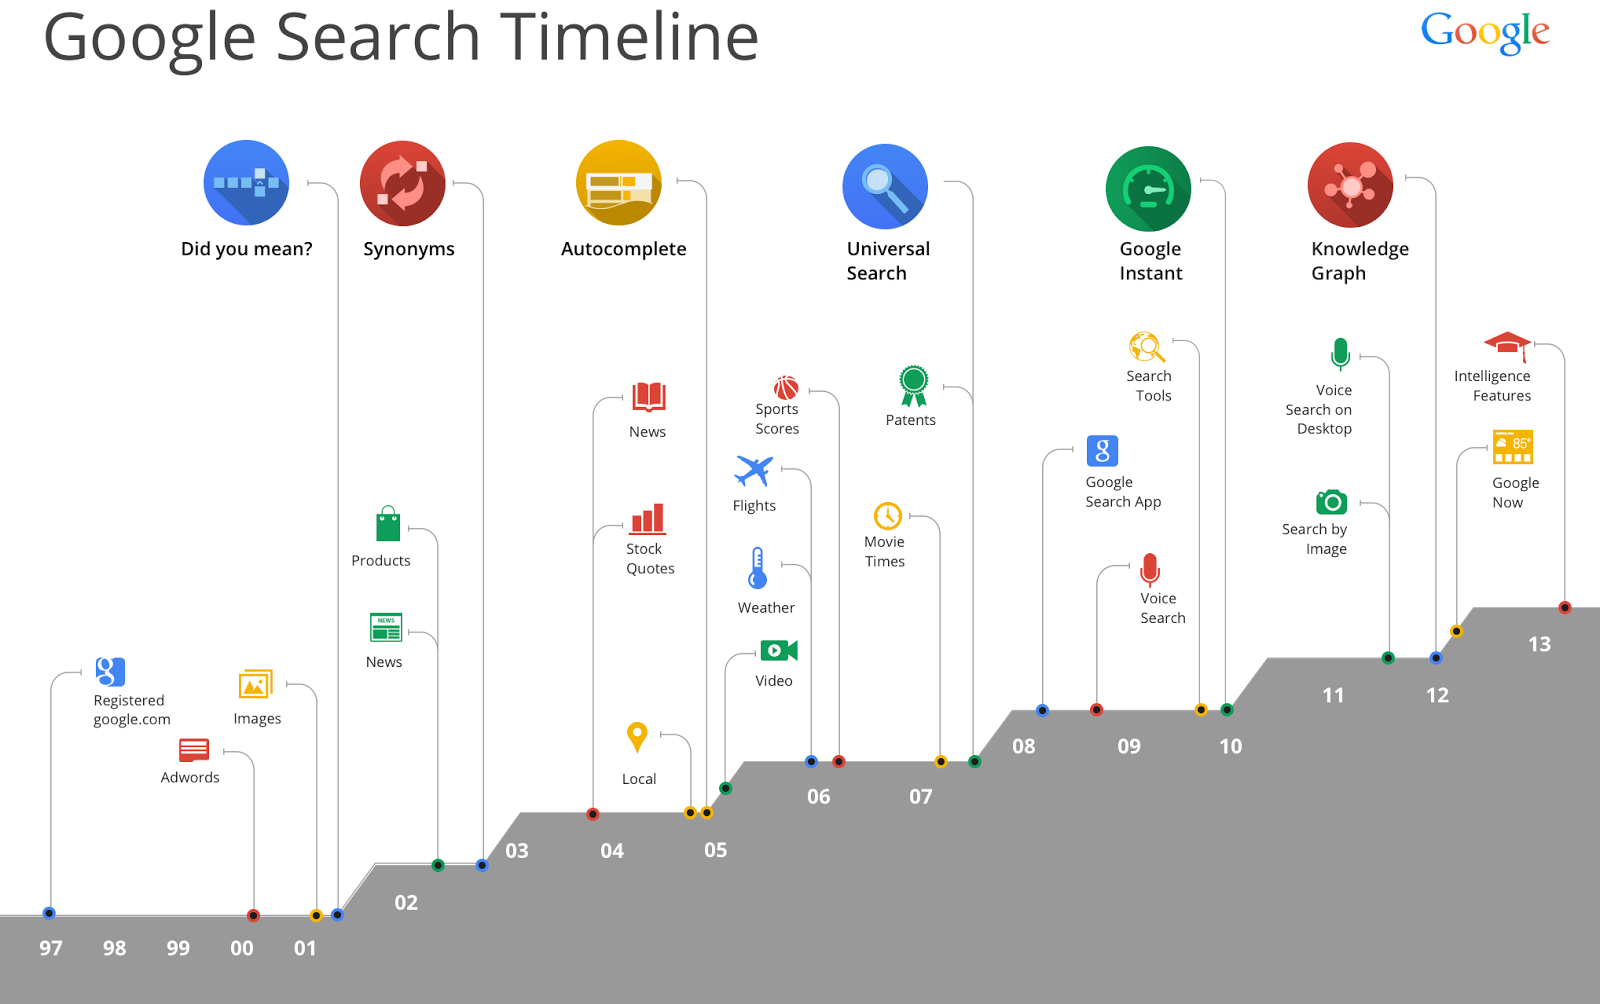
\includegraphics[width=0.6\textwidth]{Images/googleGeneration}
\end{figure}
Now are available "devices $2.0$", that have their IDs, communication capacity, computing and storage, like
for example car with maps, where the driver can asks (using text or voice audio) the route for a place.

\section{Boolean retrieval model}
We consider now the first model of Information retrieval, that was mainly used on first generation of search engine,
but are also used currently in email, library catalog and so on.

\begin{defi}
The boolean retrieval model is a model able to asks query formed by a boolean expression (query where we use 
AND, OR, NOT operators to join terms) where we views each document as a set of words and it is a precise model,
because document matches condition or not.
\end{defi}

We consider as example to determine which plays of Shakespeare contain the words 
"Brutus AND Ceaser AND NOT Calpurnia" and the simplest form is do a sort of linear scan, but this type
of text processing does not enable to rank results, consider some similarity measures and so on, so we use 
our boolean retrieval model defined above.

We consider as \emph{documents} whatever units we have
decided to build a retrieval system over, so they might be individual memos or chapters of a book.\newline
We will refer to the group of documents over which we perform retrieval as the
(document) \emph{collection} and it is sometimes also referred to as a \emph{corpus} (a body of texts).

To assess the effectiveness of an IR system (the quality of its search results), a user will usually want
to know two key statistics about the system’s returned results for a query:
\begin{description}
    \item [Precision: ] What fraction of the returned results are relevant to the information need?
    \item [Recall: ]    What fraction of the relevant documents in the collection were returned by the system?
\end{description}

In figure \ref{img:booleanMatrix} is possible to note a term-document incident matrix, where we 
record for each document, here a play of Shakespeare’s, whether it contains each word 
out of all the words Shakespeare used (Shakespeare used about 32,000 different words).

\begin{figure}
    \caption{A term-document incidence matrix. Matrix element $(t, d)$ is $1$ if the play in column $d$
             contains the word in row $t$, and is $0$ otherwise}
    \label{img:booleanMatrix}
    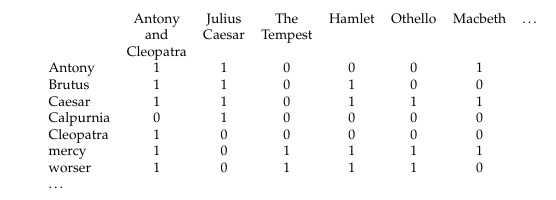
\includegraphics[width=\textwidth]{Images/booleanMatrix}
\end{figure}
The problem of Term-document incident matrix is that the matrix could be very big and it is also a \emph{sparse}
matrix, so we waste a lot of spaces to represent useless data.

To solve this problem we introduce \emph{inverted index}, where for each term $t$, we must store a list 
of all documents that contain $t$ and we identify each by docID, a document serial number.\newline
It is called inverted because usually in a document we have a list of word instead in our index we have 
for a word a list of documents where it occurs.\newline
In figure \ref{img:invertedIndex} is possible to note an example of inverted index, where we only store the docID
where a word appear in a document.

\begin{figure}
    \caption{an example of Inverted index for Brutus, Caesar and Calpurnia}
    \label{img:invertedIndex}
    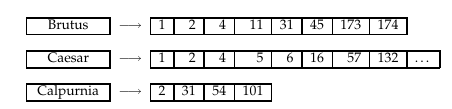
\includegraphics[width=\textwidth]{Images/invertedIndex}
\end{figure}
The advantages of inverted index is that query requires just a scan and also we can store smaller integers,
using \emph{gap coding}, that will enable to use less amount of memory.

To execute an AND query the first approach consist to check each element of the two postings list that will cause 
$n * m$ operations, where $n$ and $m$ are the length of the two postings list, and we can achieve a better result
if we sort the two postings list, so at least if we compare $1$ and $2$ we can avoid to consider to compare the
element $1$ with element that are greater than $2$, so we need only $n + m$ comparison that will improve the
performance of AND query.


The pseudocode to intersect two postings list in a AND query can be found on figure \ref{alg:intersection} and
in case we have to compute an AND query between 3 operands, it is better to first compute an AND query between
operands with smallest length and then compute an AND query with the other operand, so to compute the 
query "Brutus AND Caesar AND Calpurnia" in figure \ref{img:andQuery} we first compute "Brutus AND Calpurnia" and
then compute "(Brutus AND Calpurnia) AND Caesar"

\begin{figure}
    \caption{Pseudocode of Intersection between two postings list}
    \label{alg:intersection}
    \begin{codebox}
        \Procname{$\proc{intersection} (p_1, p_2)$}
        \li $\id{answer} \gets <> $
        \li \While $p_1 \neq \const{nil}$ and $p_2 \neq \const{nil}$ 
            \Do
        \li     \If $\proc{docID}(p_1) \isequal \proc{docID}(p_2)$
        \li         \Then $\proc{Add}(\id{answer}, \proc{docID}(p_1))$
        \li               $\id{p_1} \gets \proc{next}(p_1)$
        \li               $\id{p_2} \gets \proc{next}(p_2)$
        \li     \ElseIf $\proc{docID}(p_1) < \proc{docID}(p_2)$
        \li         \Then $\id{p_1} \gets \proc{next}(p_1)$
        \li     \Else $\id{p_2} \gets \proc{next}(p_2)$
            \End
        \li \Return $\id{answer}$
    \end{codebox}
\end{figure}
\begin{figure}
    \caption{And query between Brutus, Calpurnia and Caesar}
    \label{img:andQuery}
    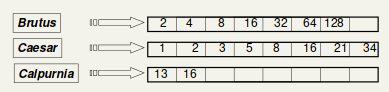
\includegraphics[width=\textwidth]{Images/andQuery}
\end{figure}
In figure \ref{alg:intersectionTerms} it can be find the pseudocode to compute the intersection between 
$n$ terms, that use the intution we have explain briefly previously.

\begin{figure}
    \caption{Pseudocode of Intersection operation between $n$ terms}
    \label{alg:intersectionTerms}
    \begin{codebox}
	\Procname{$\proc{intersection} (<t_1, \dots, t_n>)$}
	    \li $\id{terms} \gets \proc{SortByIncreasingFrequency}(<t_1, \dots, t_n>)$
	    \li $\id{result} \gets \proc{postings} (\proc{first}(\id{terms}))$
	    \li $\id{terms} \gets \proc{rest} (\id{terms})$
	    \li \While $\id{terms} \neq \const{nil}$ and $\id{result} \neq \const{nil}$
	    	\Do
	    \li $\id{result} \gets \proc{intersect} (\id{result}, postings(\proc{first} (\id{terms})))$
	    \li $\id{terms} \gets \proc{rest} (\id{terms})$
	        \End
	    \li \Return $\id{result}$
    \end{codebox}
\end{figure}
To gain the speed benefits of indexing at retrieval time, we have to build the index in advance
and the major steps in this are:
\begin{enumerate}
    \item Collect the documents to be indexed
    \item Tokenize the text, turning each document into a list of tokens
    \item Do linguistic preprocessing, producing a list of normalized tokens, which are the indexing terms
    \item Index the documents that each term occurs in by creating an inverted index,
          consisting of a dictionary and postings
\end{enumerate}
The first three steps will consider later in the course and the last one is considered now when we talk about 
inverted index.

To represent the index we have to done some choice about data structure to use, infact 
a fixed length array would be wasteful as some words occur in many documents, and others in very few.\newline
For an in-memory postings list, two good alternatives are singly linked lists or variable length arrays:
singly linked lists allow cheap insertion of documents into postings lists (following updates,
such as when recrawling the web for updated documents), and naturally extend to more advanced indexing strategies
such as skip lists, which require additional pointers.\newline
Variable length arrays win in space requirements by avoiding the overhead for pointers and in
time requirements because their use of contiguous memory increases speed on modern processors with memory caches
and extra pointers can in practice be encoded into the lists as offsets.

If updates are relatively infrequent, variable
length arrays will be more compact and faster to traverse and we can also use a
hybrid scheme with a linked list of fixed length arrays for each term.\newline
When postings lists are stored on disk, they are stored (perhaps compressed) as a
contiguous run of postings without explicit pointers 
to minimize the size of the postings list and the number of disk seeks to read
a postings list into memory.

An improvement to our intersection can be obtained with \emph{skip pointers}, where we put a pointer 
head to some element that will permits to avoid to consider some elements, as it can be viewed on 
figure \ref{img:skip} and in figure \ref{alg:skip} there is the pseudocode of intersection with skip pointers.


\begin{figure}
    \caption{Postings lists with skip pointers. The postings intersection can use a skip pointer
             when the end point is still less than the item on the other list.}
    \label{img:skip}
    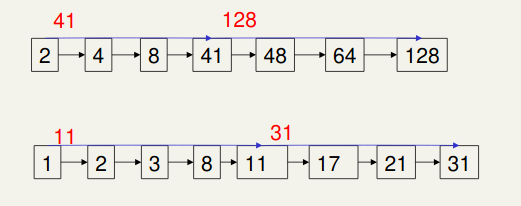
\includegraphics[width=\textwidth]{Images/skip}
\end{figure}

\begin{figure}
    \caption{Pseudocode of Intersection with Skip Pointers}
    \label{alg:skip}
    \begin{codebox}
	\Procname{$\proc{intersectWithSkips} (p_1, p_2)$}
	\li $\id{answer} \gets <>$
	\li \While $p_1 \neq \const{nil}$ and $p_2 \neq \const{nil}$
	    \Do
	\li        \If $\proc{docID}(p_1) = \proc{docID}(p_2)$
	    	   \Then
	\li 	          
    \end{codebox}
\end{figure}
With skip we can logically divide elements in block, where we can access to the first item of a block and we 
can avoid maybe avoid to consider other elements of a block.\newline
The important thing that we have to record is that more is the size of a block less is the number of skip pointers 
and more element is possible to purge from our operation and we have as worst case when all elements are 
in the last block so we have to consider $\frac{n}{L}$ blocks and $L$ to scan the last block and we achieve 
\[ min \frac{n}{L} + L \]
when $L = \sqrt{n}$.

Typically we use a dynamic programming based skip pointers, where we assume that exist some documents 
very frequent as a result of a query so whenever we do an intersection it is more likely that they are occuring,
so we divide block with frequent document as start of a block.\newline
With Dynamic Programming approach the append of a new element will be difficult because we have to recompute
the distribution of skip pointers instead on equal size skip pointers we only append new block, with the new element.

Another improvement is \emph{Recursive Merge}, where we take a pivot (the median element) and we do a 
binary search to retrieve if the pivot occurs in the other lists and then we do something similar to Quicksort.\newline
The time complexity of this approach is the following:
\begin{description}
    \item [Best Case: ] we have that the median is always out of the other list so we have $O(\log n * \log m)$, 
	                because you always remove the upper bound of the list so we consider only the lower bound of median.
    \item [Worst Case: ] we have that median is always inside the list so we have 
			 \[ T(n, m) = O(\log n) + 2T(n/2, m/2) = O(m \log n/m) \]
			 where the last equation is obtained by master theorem.
\end{description}
If $m \sim n$ we have $O(m) = O(n + m)$, in case $m << n$ we obtain $O(m \log n)$ that means for every element in list
of size $m$ we do a binary search.

In case we have an OR query we do an union between $n$ posting list without problem, instead with an OR NOT query
there will be a problem because if we have a list with $2$ element the complementation of a list has $N - 2$ 
elements and that will be a huge problem. 

Information Retrieval is not only limited to boolean model so we want to consider phrases, proximity operators
like "Gates near Microsoft" where we need index to capture term position in docs and sometimes we are also 
interested to consider zones in documents like "Find documents with (author = Ullman) and (text contains automata)".

We define zone indexes as
\begin{defi}
    Zone indexes: is a region of the doc that can contain an arbitrary amound of text, like title, abstract
                  or references.
\end{defi}
We build inverted indexes on fields and zones to permit querying, as can be noted on figure \ref{img:zoneIndex}.

\begin{figure}
    \caption{Inverted index on zone fields}
    \label{img:zoneIndex}
    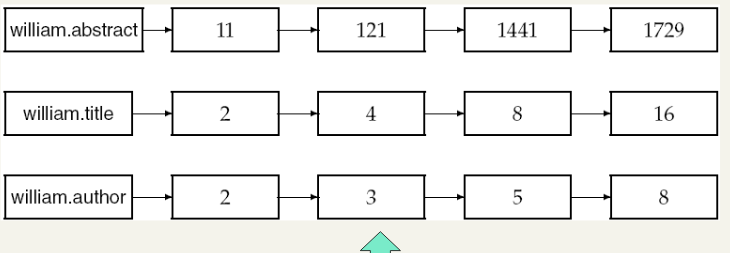
\includegraphics[width=\textwidth]{Images/zoneIndex}
\end{figure}

An \emph{search engine} it comes of several components that can be viewed in figure \ref{img:searchEngine}, 
we will start talking about crawling and then we will introduce the other components in the following chapter.

